%%%%%%%%%%%%%%%%%%%%%%%%%%%%%%%%%%%%%%%%%
% Dreuw & Deselaer's Poster
% LaTeX Template
% Version 1.0 (11/04/13)
%
% Created by:
% Philippe Dreuw and Thomas Deselaers
% http://www-i6.informatik.rwth-aachen.de/~dreuw/latexbeamerposter.php
%
% This template has been downloaded from:
% http://www.LaTeXTemplates.com
%
% License:
% CC BY-NC-SA 3.0 (http://creativecommons.org/licenses/by-nc-sa/3.0/)
%
%%%%%%%%%%%%%%%%%%%%%%%%%%%%%%%%%%%%%%%%%

%----------------------------------------------------------------------------------------
%	PACKAGES AND OTHER DOCUMENT CONFIGURATIONS
%----------------------------------------------------------------------------------------

\documentclass[final, hyperref={pdfpagelabels=false}]{beamer}

\usepackage[orientation=portrait,size=a0,scale=1.4]{beamerposter-v2} % Use the beamerposter package for laying out the poster with a portrait orientation and an a0 paper size
\usetheme{I6pd2-v2} % Use the I6pd2 theme supplied with this template
\usepackage{booktabs} % Top and bottom rules for tables
\usepackage[english]{babel} % English language/hyphenation
\usepackage{verbatim}
\usepackage{setspace}
% \usepackage[framemethod=tikz]{mdframed}

\usepackage{amsmath,amsthm,amssymb,latexsym} % For including math equations, theorems, symbols, etc
\newcommand{\defeq}{\mathrel{\stackrel{\text{def}}{=}}}
\newcommand{\musteq}{\mathrel{\stackrel{\text{!}}{=}}}
\DeclareMathOperator{\Imag}{Im}
\DeclareMathOperator{\diag}{diag}
\DeclareMathOperator{\Span}{span}
\DeclareMathOperator{\Col}{col}


\makeatletter
\def\input@path{{figures/}}
\makeatother
\graphicspath{{figures/}} % Location of the graphics files

\usepackage{xcolor}
\definecolor{tabutter}{rgb}{0.98824, 0.91373, 0.30980}		% #fce94f
\definecolor{taorange}{rgb}{0.98824, 0.68627, 0.24314}		% #fcaf3e
\definecolor{ta2orange}{rgb}{0.96078, 0.47451, 0}		% #f57900
\definecolor{ta3orange}{rgb}{0.80784, 0.36078, 0}		% #ce5c00

%\usepackage{pgf}
\usepackage{tikz}
\usepackage{gnuplot-lua-tikz}
\usetikzlibrary{decorations.pathmorphing, decorations.pathreplacing, decorations.text}
\usetikzlibrary{arrows.meta}
\usetikzlibrary{shapes, shapes.symbols, shapes.geometric}
\usetikzlibrary{automata}
\usetikzlibrary{positioning}
\usetikzlibrary{calc}
\usetikzlibrary{bending}
\usetikzlibrary{matrix}
\usetikzlibrary{backgrounds,fit}
\tikzstyle{every picture}+=[remember picture]
\everymath{\displaystyle}

%----------------------------------------------------------------------------------------
%	TITLE SECTION
%----------------------------------------------------------------------------------------

\title{%\VERYHuge
{\Huge Calculating Non-resonant Inelastic X-ray
} \\ \Huge Spectra from First Principles } % Poster title

\author{\texorpdfstring{\underline{Maxime Vinteler}$^{\ast}$}{Maxime Vinteler}\inst{1} \and Benjamin Lenz\inst{1} \and  Guillaume Radtke\inst{1} \and Coraline Letouz\'e\inst{1}}

\institute{
\inst{1} Institut de Min\'eralogie, de Physique des Mat\'eriaux et de Cosmochimie, Sorbonne Universit\'e, UMR CNRS 7590,\\Mus\'eum National d'Histoire Naturelle, 75005 Paris, France
\medskip

$^*$ Corresponding author: \href{mailto:maxime.vinteler@etu.sorbonne-universite.fr}{maxime.vinteler@etu.sorbonne-universite.fr}
}

\begin{document}

\addtobeamertemplate{block end}{}{\vspace*{1em}} % White space under blocks

\begin{frame}[t] % The whole poster is enclosed in one beamer frame


%%%%%%%%%%%%%%%%%%%%%%%%%%%%%%%%%%%%%%%%%%%%%%%%%%%%%%%%%%%%%%%%%%
%MOTIVATION & HUBBARD MODEL
%%%%%%%%%%%%%%%%%%%%%%%%%%%%%%%%%%%%%%%%%%%%%%%%%%%%%%%
\vspace{-0.75em}


\begin{columns}[t]  % beginning of all the columns

\begin{column}{.03\textwidth}
\end{column} % Empty spacer column

\begin{column}{.60\textwidth} % The first column
\begin{block}{\color{ta2orange!0}Motivation}
\setbeamercolor{coloredboxstuff}{bg=ta2orange!0}
\begin{beamercolorbox}[wd=\textwidth]{coloredboxstuff}
Non-resonant inelastic x-ray scattering (NRIXS) gives access to the orbital shape of the hole-part of the material’s ground state \cite{Yavas2019, Baledent}. Here, we aim to compute it from \textit{ab initio} methods for CuO.

\vspace{0.5em}

\begin{minipage}[c]{0.3\textwidth}
\vspace{-1.em}
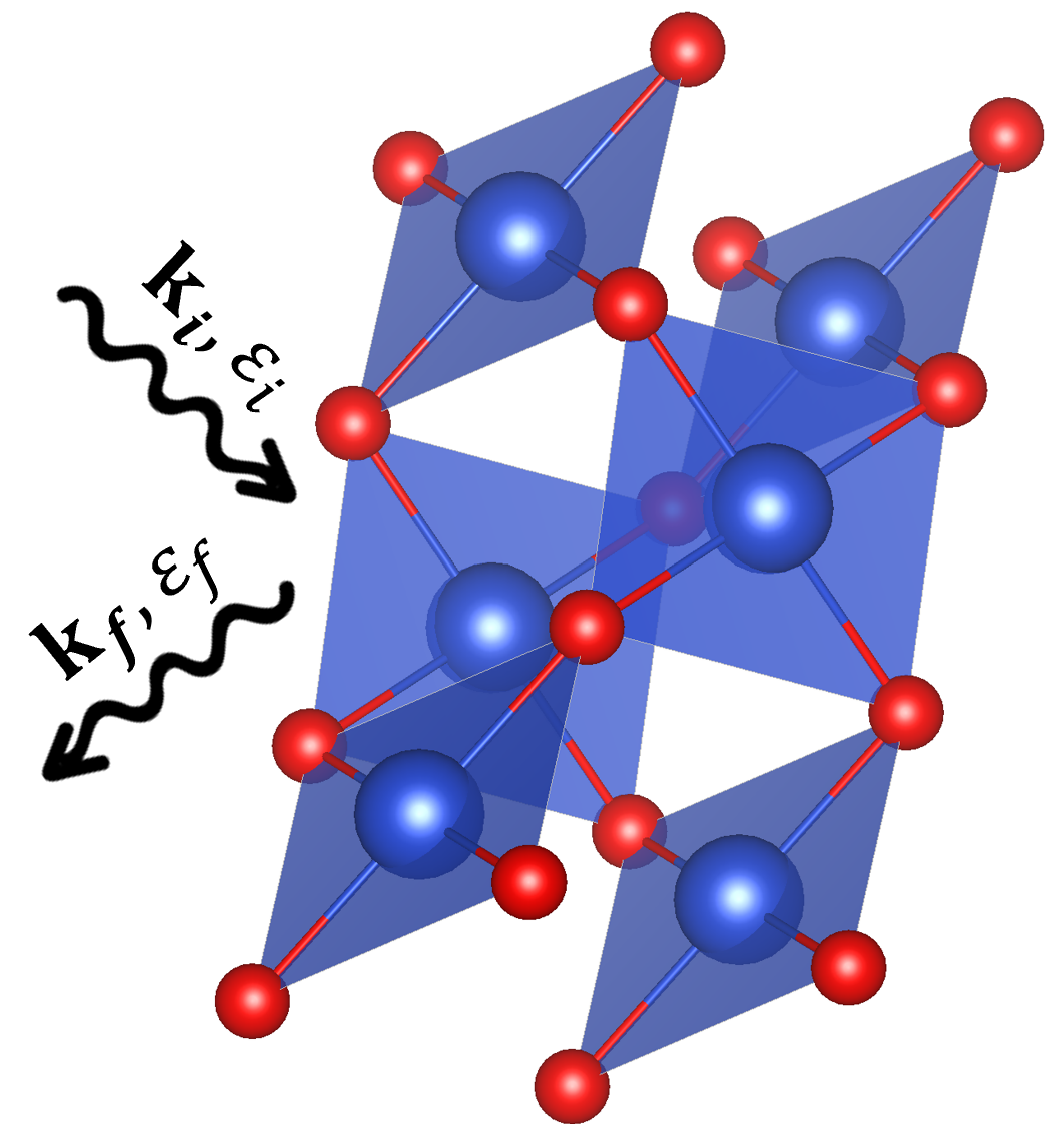
\includegraphics[width=0.7\textwidth]{imgs/CuO_v2.png}
\end{minipage}
%
\hspace{-1.5em}
%
\begin{minipage}[c]{0.3\textwidth}
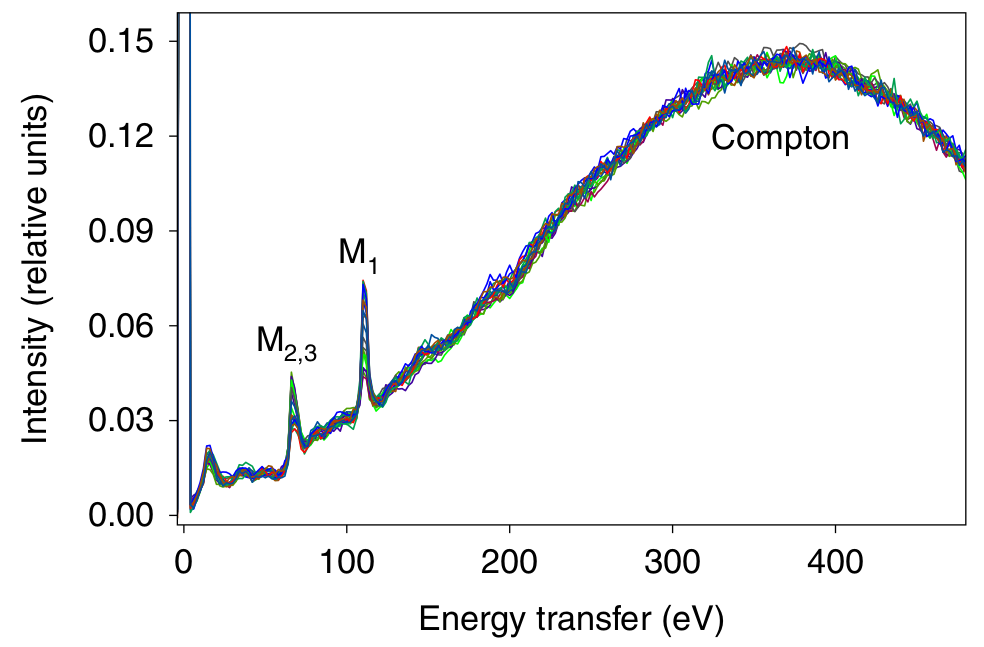
\includegraphics[width=1.3\textwidth]{imgs/NRIXS_NiO_spectra.png}
\end{minipage}
%
\hfill
%
\begin{minipage}[c]{0.33\textwidth}
\hspace{3em}
\vspace{1.05em}
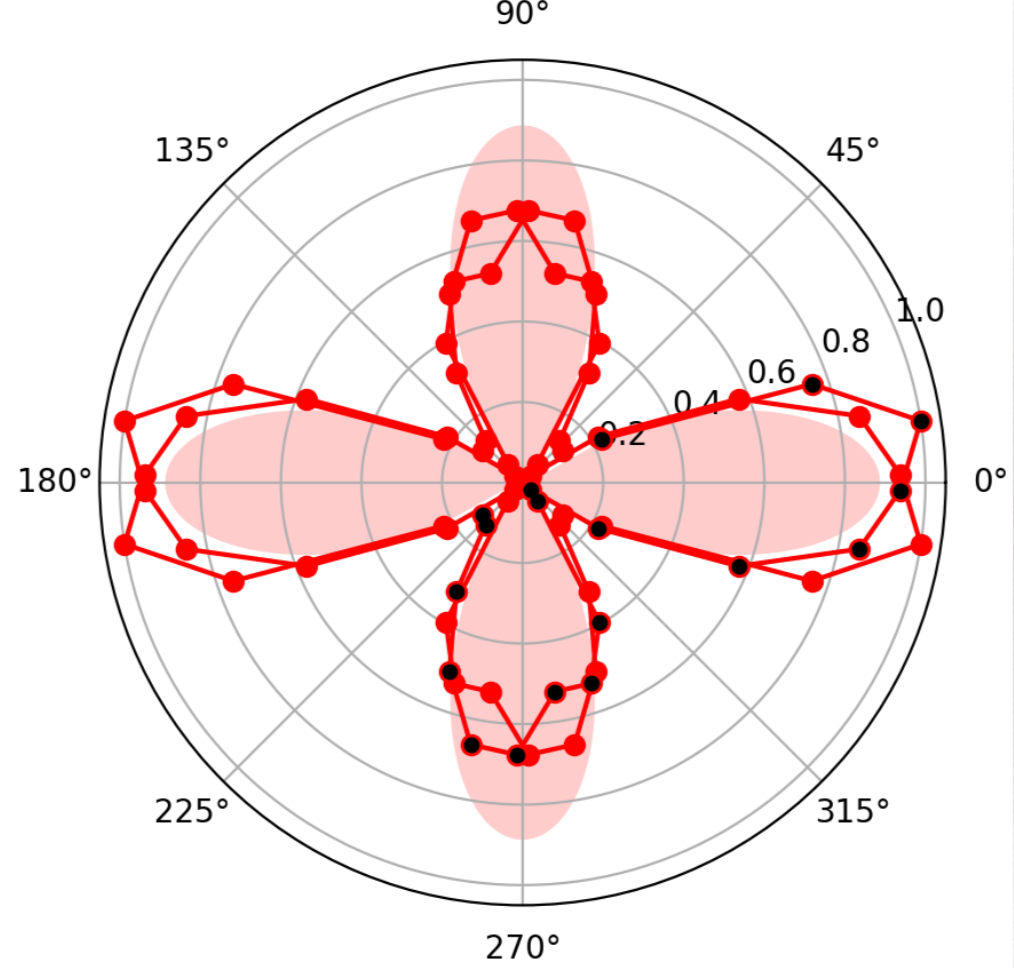
\includegraphics[width=0.75\textwidth]{imgs/victor_results.png}
\end{minipage}

\vspace{0.5em}

The $\text{M}_1$ edge can be used to probe quadrupole 3s $\rightarrow$ 3d electronic transitions. The angular dependence is then  dictated by the final state and we can therefore get an image of the $\text{Cu}^{2+}$ hole.
\end{beamercolorbox}
\end{block}
\end{column}

\begin{column}{.02\textwidth}
\end{column}	%Empty spacer column in the middle
\begin{column}{.34\textwidth}
\begin{block}{\color{ta2orange!0} Hubbard model}
\setbeamercolor{coloredboxstuff}{bg=ta2orange!0}
\begin{beamercolorbox}[wd=\textwidth]{coloredboxstuff}
Copper oxide being a \textbf{strongly correlated material}, an appropriate first approximation model is the \textbf{one orbital Hubbard model} :

\vspace{0.1em}
\begin{equation*}
\hat{H} = -\sum_{ij\sigma} t_{ij} c_{i\sigma}^{\dagger}c_{j\sigma}^{\phantom{\dagger}} + U \sum_{i} n_{i\uparrow} n_{i\downarrow}
\end{equation*}
\vspace{0.1em}

where $t_{ij}$ is the hopping amplitude between sites $i$ and $j$, which tends to delocalize the electrons, and $U$ is the on-site Coulomb repulsion, which favors their localization.

\vspace{1.1em}

But which orbital should we choose? How can we compute $t_{ij}$ and $U$ for CuO? And how can we solve this model numerically ?
\end{beamercolorbox}
\end{block}
\end{column}

\begin{column}{.03\textwidth}
\end{column} % Empty spacer column

\end{columns} % End of all the columns
\vspace{-0.75em}


%%%%%%%%%%%%%%%%%%%%%%%%%%%%%%%%%%%%%%%%%%%%%%%%%%%%%%%%%%%%%%%%%%
% DFT & WANNIER
%%%%%%%%%%%%%%%%%%%%%%%%%%%%%%%%%%%%%%%%%%%%%%%%%%%%%%%


\begin{columns}[t] % The whole poster consists of two major columns, each of which can be subdivided further with another \begin{columns} block - the [t] argument aligns each column's content to the top

\begin{column}{.03\textwidth}
\end{column} % Empty spacer column

\begin{column}{.53\textwidth} % The first column
\begin{block}{\color{cyan!40} Density Functional Theory (DFT)}
\setbeamercolor{coloredboxstuff}{bg=cyan!5}
\begin{beamercolorbox}[wd=\textwidth]{coloredboxstuff}

DFT is a mean-fied, ground-state theory. It allows to compute the Bloch states (BS), the bands (right) and the density of states (left) of CuO with projected Cu-3d/4s and O-2p.

\vspace{0.15em}

	\begin{minipage}{0.42\textwidth}
	\centering
	
\includegraphics[width=1.3\textwidth]{imgs/dos_vs_bands_v1.pdf}
   \end{minipage}
   \hspace{4.5em}
   	\begin{minipage}{0.43\textwidth}
Near the Fermi level: \textbf{four conduction bands of Cu-$\mathbf{3d_{x^2-y^2}}$ character} (from crystal field splitting), hybridized with O-2p orbitals.

\vspace{1.4em}

Bands partially filled, yet CuO is insulating in experiments
\begin{center}
$\Rightarrow$ \textbf{correlation effects}
\end{center}
   \end{minipage}
\end{beamercolorbox}
\end{block}
\end{column} % End of the middle column
\begin{column}{.017\textwidth}
\end{column}	%Empty spacer column in the middle

\begin{column}{.40\textwidth}
	\begin{block}{\color{cyan!40} Wannier Functions (WF)}
	\setbeamercolor{coloredboxstuff}{bg=cyan!5}
	\begin{beamercolorbox}[wd=\textwidth]{coloredboxstuff}
WF are Fourier transform of the BS : $\left| \textbf{R}n \right> = \int_{\text{BZ}} \text{d}\textbf{k} \; e^{-i\textbf{k}\textbf{R}} \left| \phi_{n,\textbf{k}} \right>.$

\vspace{-0.5em}

\begin{minipage}{0.53\textwidth}
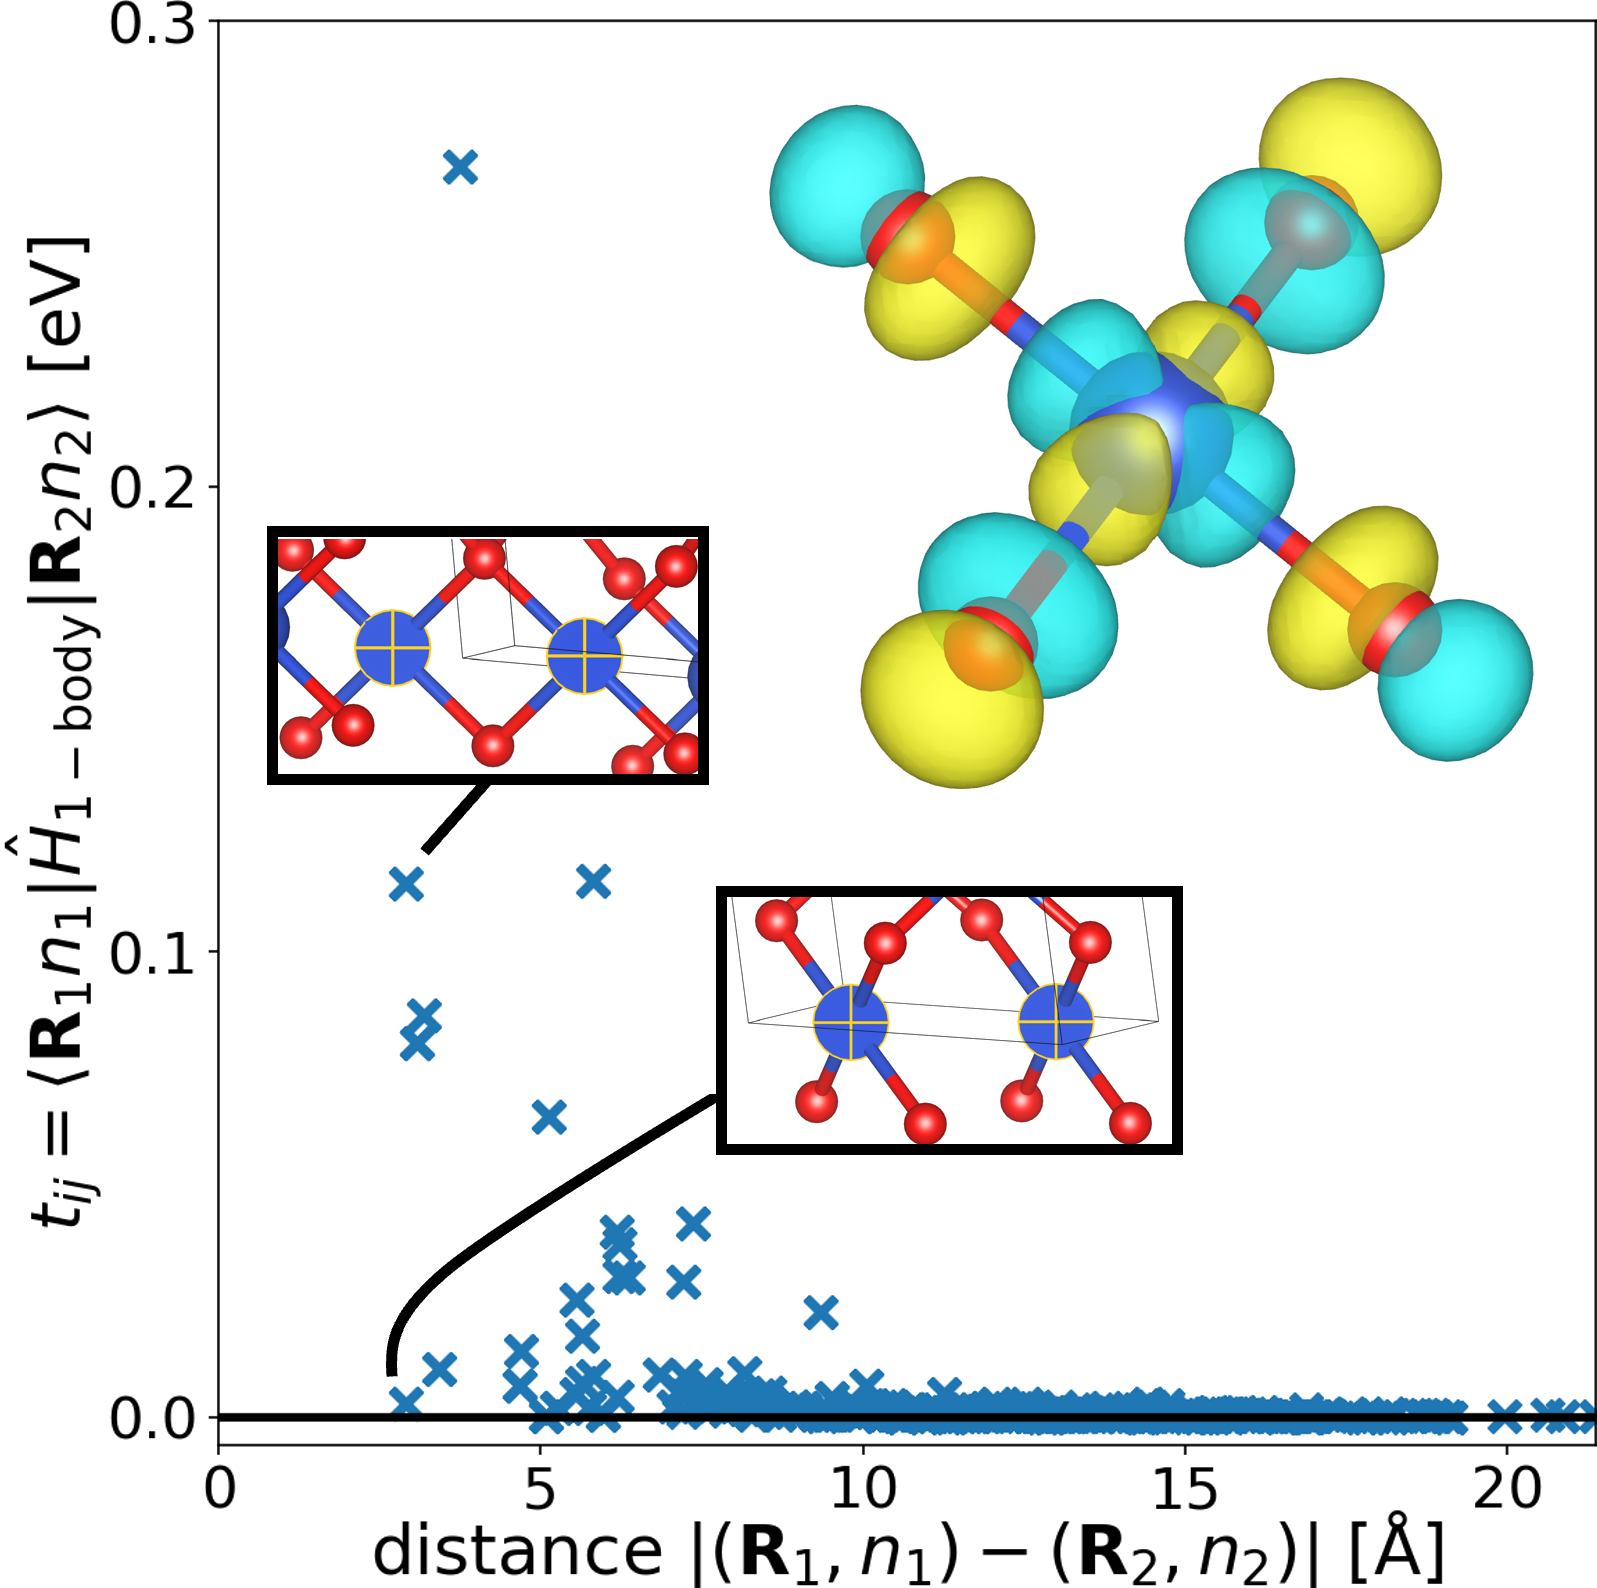
\includegraphics[width=0.985\textwidth]{imgs/hopping_terms_v4.png}
\end{minipage}
\hfill
\begin{minipage}{0.45\textwidth}
These WF are localized $\text{3d}_{x^2-y^2}$ orbitals centered on each of the four copper atoms at lattice vector \textbf{R} (see top-right image).

\vspace{1.5em}

Combination with the neighboring oxygen 2p orbitals, with $\sigma$-type overlaps
\end{minipage}
	\end{beamercolorbox}
	\end{block}
\end{column}

\begin{column}{.03\textwidth}
\end{column} % Empty spacer column
\end{columns} % End of all the columns in the poster
\vspace{-0.75em}


%%%%%%%%%%%%%%%%%%%%%%%%%%%%%%%%%%%%%%%%%%%%%%%%%%%%%%%%%%%%%%%%%%
%CRPA & DMFT
%%%%%%%%%%%%%%%%%%%%%%%%%%%%%%%%%%%%%%%%%%%%%%%%%%%%%%%


\begin{columns}[t] % The whole poster consists of two major columns, each of which can be subdivided further with another \begin{columns} block - the [t] argument aligns each column's content to the top

\begin{column}{.03\textwidth}
\end{column} % Empty spacer column

\begin{column}{.35\textwidth} % The first column
\begin{block}{\color{cyan!40} constrained Random Phase Approx.\vphantom{Dy)}}
\setbeamercolor{coloredboxstuff}{bg=cyan!5}
\begin{beamercolorbox}[wd=\textwidth]{coloredboxstuff}

\textbf{Screening potential} : $W(\mathbf{r},\mathbf{r'}) = \left( 1 - vP_0^r\right)^{-1}v$

\vspace{0.5em}

\begin{minipage}{0.4\textwidth}
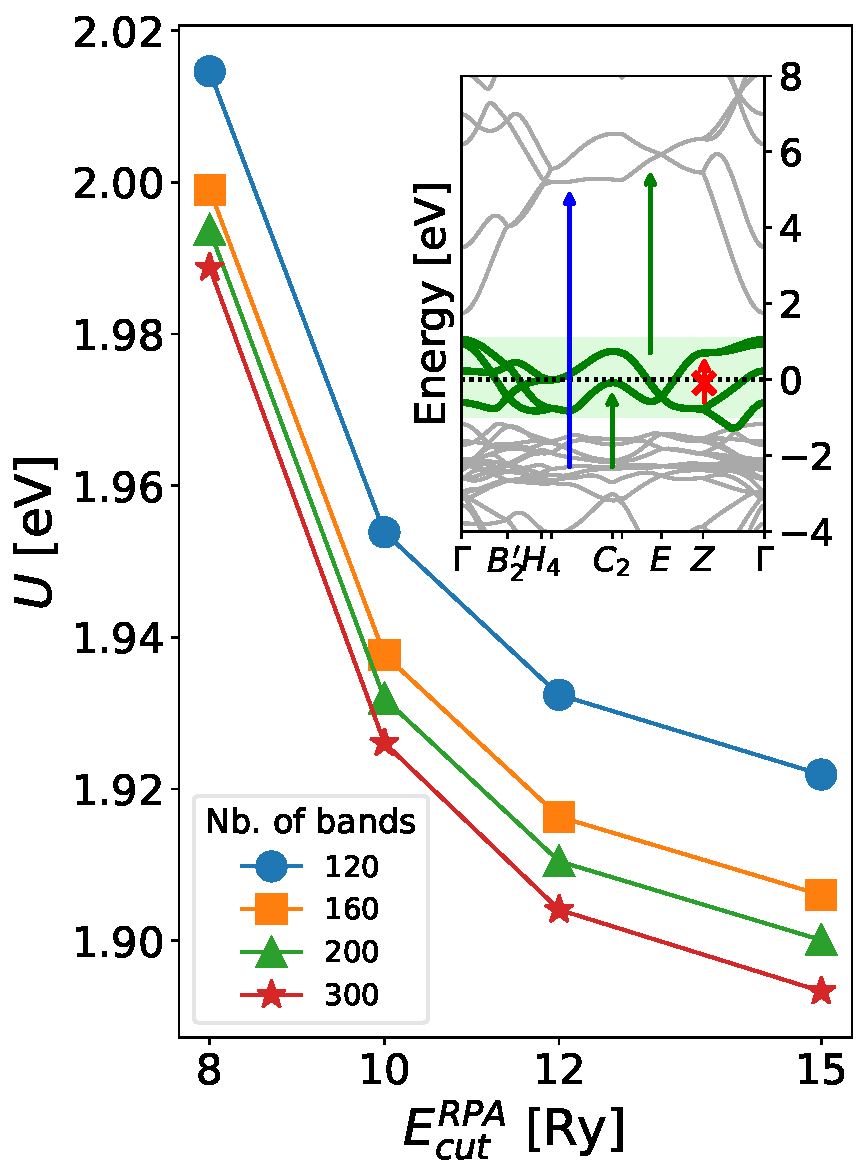
\includegraphics[width=1.145\textwidth]{imgs/cRPA_conv.pdf}
\end{minipage}
\hfill
\begin{minipage}{0.52\textwidth}

\vspace{-1em}

$v$ : bare Coulomb interaction

\vspace{0.5em}

$P_0^r$ : response function of $W$ calculated using cRPA.\\
Allowed transitions: outside the $d$-subspace (top right figure) and below $E_{\text{cut}}^{\text{RPA}}$.

\vspace{1em}

\textbf{Convergence graph}\\
$U = 1.9$ eV for $200$ bands and $15$ Ry cutoff --- value used in the following.
\end{minipage}

\end{beamercolorbox}
\end{block}
\end{column} % End of the middle column

\begin{column}{.017\textwidth}
\end{column}	%Empty spacer column in the middle

\begin{column}{.58\textwidth}
	\begin{block}{\color{cyan!40} Dynamical Mean Field Theory (DMFT)}
	\setbeamercolor{coloredboxstuff}{bg=cyan!5}
	\begin{beamercolorbox}[wd=\textwidth]{coloredboxstuff}

DMFT maps the lattice problem self-consistently onto an impurity model \cite{Georges1996}, solved with \textsc{triqs} \& \textsc{cthyb} \cite{Seth2016}, at $T=290$ K in a paramagnetic phase (see right: imaginary part of the self-energy).

\vspace{0.5em}

\begin{minipage}{0.61\textwidth}
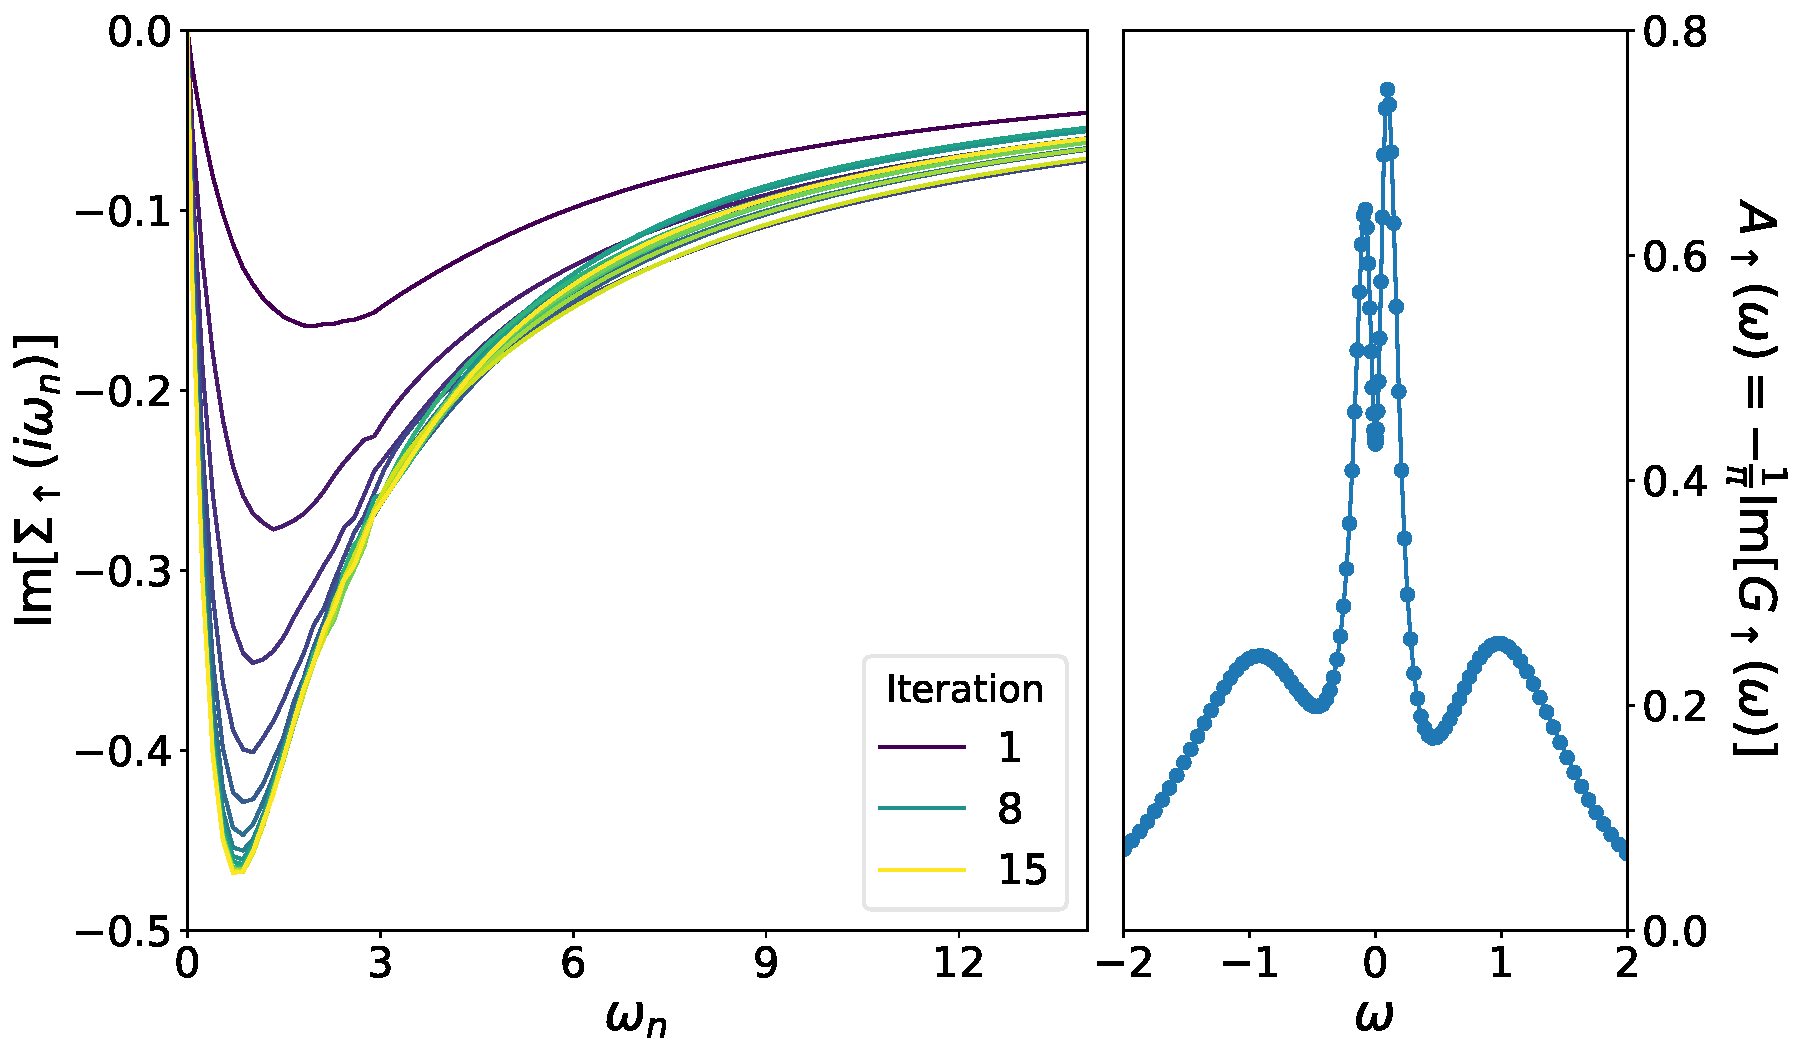
\includegraphics[width=0.96\textwidth]{imgs/self_spec.pdf}
\end{minipage}
\hfill
\begin{minipage}{0.381\textwidth}
\vspace{-0.9em}
Analytic continuation from imaginary to real frequencies using \textsc{MaxEnt} \cite{maxent}\\ $\rightarrow$ spectral function $A(\omega)$ (right).

\vspace{1.5em}

\textbf{Non zero Spectral weight at} $\mathbf{\omega = 0}\Rightarrow$ \textbf{Bad metal phase.}\\
\underline{Reason} : overscreening of cRPA or missing antiferromagnetism ?
\end{minipage}

	\end{beamercolorbox}
	\end{block}
\end{column}

\begin{column}{.03\textwidth}
\end{column} % Empty spacer column
\end{columns} % End of all the columns in the poster
\vspace{-0.75em}

%%%%%%%%%%%%%%%%%%%%%%%%%%%%%%%%%%%%%%%%%%%%%%%%%%%%%%%%%%%%%%%%%%
%PHASE DIAGRAM & ONGOING DEVELOPMENTS
%%%%%%%%%%%%%%%%%%%%%%%%%%%%%%%%%%%%%%%%%%%%%%%%%%%%%%%


\begin{columns}[t]  % beginning of all the columns

\begin{column}{.03\textwidth}
\end{column} % Empty spacer column

\begin{column}{.52\textwidth} % The first column
\begin{block}{\color{ta2orange!30!tabutter!30} Phase Diagram of CuO\vphantom{Xy}}
\setbeamercolor{coloredboxstuff}{bg=ta2orange!10!tabutter!10}
\begin{beamercolorbox}[wd=\textwidth]{coloredboxstuff}

We computed the phase diagram of CuO in the paramagnetic and antiferromagnetic phase to choose the best parameters $(U, T)$ that describe the insulating phase.

\vspace{0.5em}

\hspace{0.7em}
\begin{minipage}{0.46\textwidth}
\centering
Paramagnetic DMFT
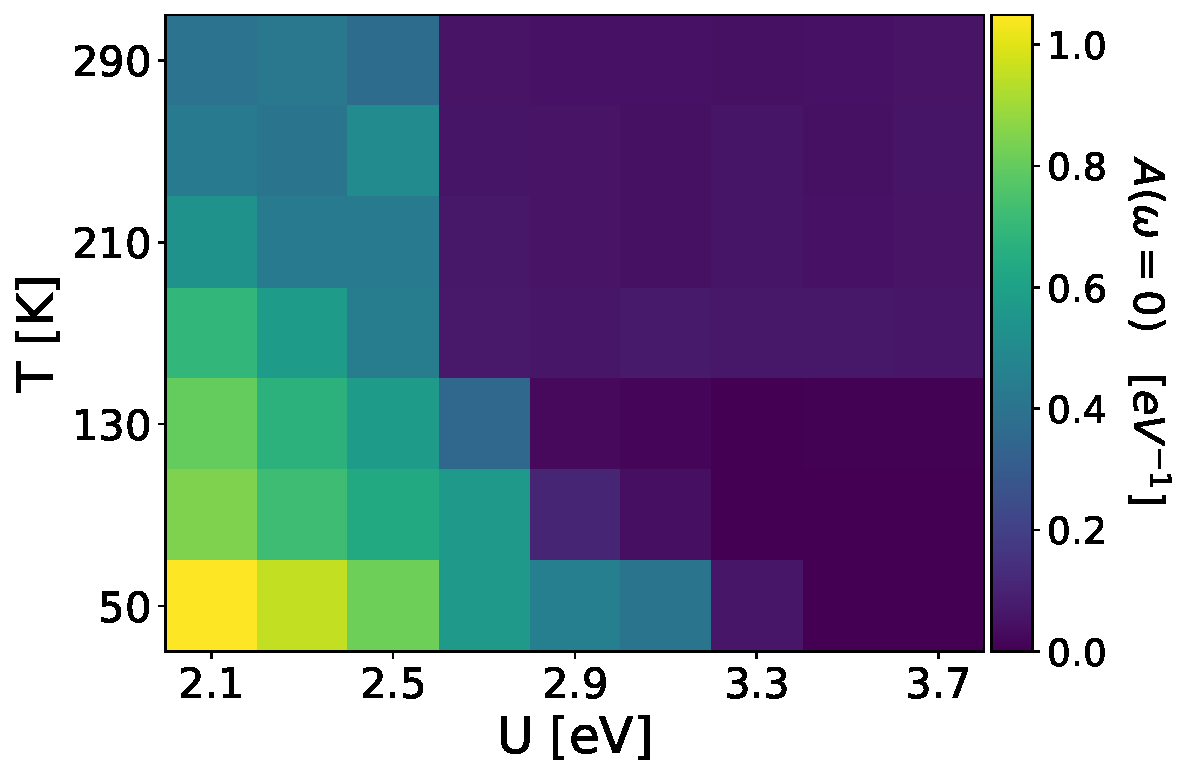
\includegraphics[width=1\textwidth]{imgs/phase_diag_para.pdf}
\end{minipage}
\hspace{0.5em}
\begin{minipage}{0.46\textwidth}
\centering
Anti-ferromagnetic DMFT
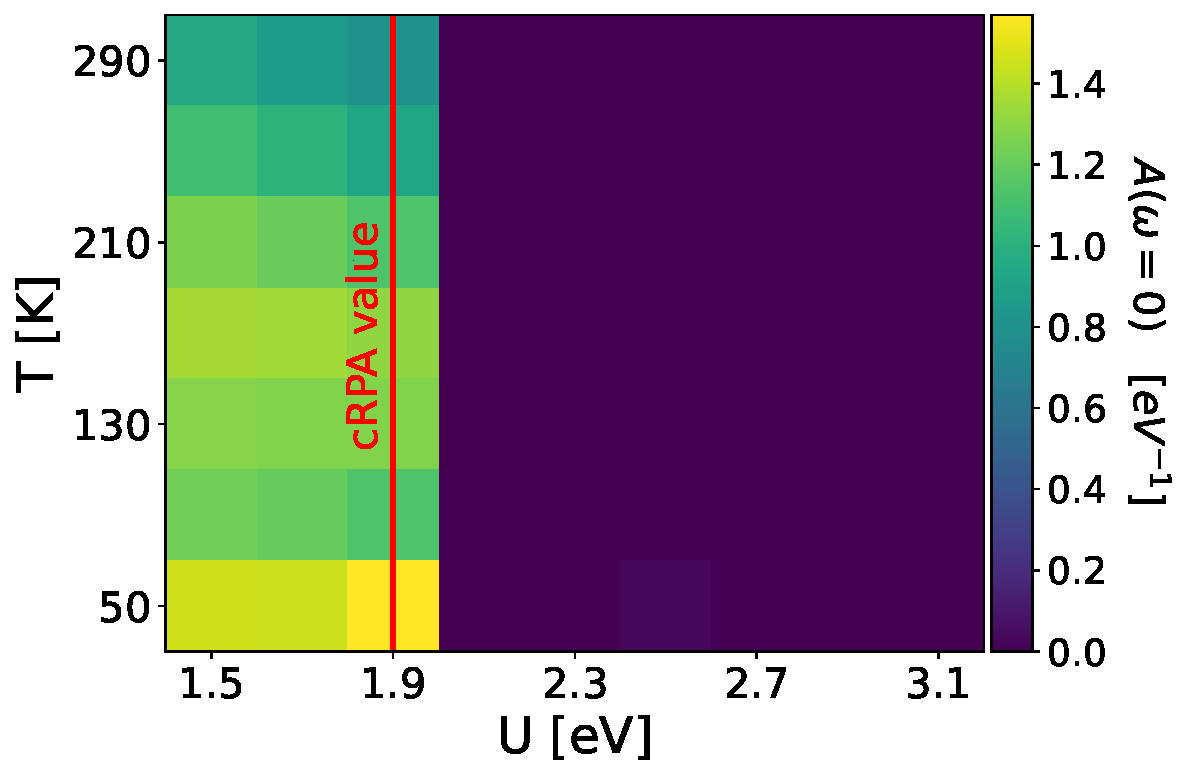
\includegraphics[width=01\textwidth]{imgs/phase_diagram_CuO_A0_AF.pdf}
\end{minipage}

\end{beamercolorbox}
\end{block}
\end{column}

\begin{column}{.02\textwidth}
\end{column}	%Empty spacer column in the middle

\begin{column}{.40\textwidth} % The first column
\begin{block}{\color{ta2orange!30!tabutter!30} Ongoing developments\vphantom{Xy}}
\setbeamercolor{coloredboxstuff}{bg=ta2orange!10!tabutter!10}
\begin{beamercolorbox}[wd=\textwidth]{coloredboxstuff}

Last remaining step is the diagonalization of the impurity Hamiltonian, taking into account quadrupole $3s \rightarrow 3d$ excitations
\vspace{0.45em}
\begin{align*}
\hat{H}_{\text{imp}} = & \overbrace{\sum_{l\sigma}^{\phantom{.}}\epsilon_la_{l\sigma}^{\dagger}a_{l\sigma}^{\phantom{\dagger}}}^{\text{bath}}+ \overbrace{\sum_{l\sigma}^{\phantom{.}}\left(V_{l\sigma}a_{l\sigma}^{\dagger}c_{\sigma}^{\phantom{\dagger}}+ \text{h.c.} \right)}^{\text{hybridization imp. - bath}} + \overbrace{E_{3s} \left( n_{3s\uparrow} + n_{3s\downarrow}\right)^{\phantom{Y}}}^{\text{core}} \\
& + \underbrace{Un_\uparrow n_\downarrow - \mu  \left( n_\uparrow + n_\downarrow \right)_{\phantom{p}}}_{\text{impurity}} + \underbrace{U_{3s,3d} \left( n_{\uparrow} n_{3s\uparrow}+n_{\downarrow} n_{3s\downarrow}\right)_{\phantom{y}}}_{\text{core-hole interaction}}
\end{align*}

\vspace{0.35em}

where $\{\epsilon_l, V_{l\sigma}, \mu \}$ are obtained from DMFT, and $\{U_{3s \rightarrow 3d}, E_{3s} \}$ are taken from the literature. These eigenenergies and eigenstates can then be used to calculate the NRIXS cross section.

\vspace{1.05em}
\end{beamercolorbox}
\end{block}
\end{column}

\begin{column}{.03\textwidth}
\end{column} % Empty spacer column
\end{columns}
\vspace{-0.75em}

%%%%%%%%%%%%%%%%%%%%%%%%%%%%%%%%%%%%%%%%%%%%%%%%%%%%%%%%%%%%%%%%%%%%%%%%%%%%%%%%%%%%%%%%%%%%%%%%%%%%%%%%%%%%%%%%%%%%%%%%%

\begin{columns}[t]  % beginning of all the columns

\begin{column}{.03\textwidth}
\end{column} % Empty spacer column

\begin{column}{0.94\textwidth}
%
\begin{block}{\color{gray!10} \normalsize References}
{\footnotesize
\begin{thebibliography}{4}

\bibitem{Yavas2019}
H. Yavas, M. Sundermann, K. Chen, A. Amorese, A. Severing, H. Gretarsson, M. W. Haverkort, and L. H. Tjeng. \textit{Direct imaging of orbitals in quantum materials. Nature Physics}, 15(6) :559–562, 2019.

\bibitem{Baledent}
Right figure of the \textit{Motivation} box : experimental results of orbital imaging of copper oxide at $300$ K, by Victor Baledent and Jean-Pascal Rueff, with whom we are collaborating. The NRIXS spectra comes from paper \cite{Yavas2019} for NiO.

\bibitem{Georges1996}
A. Georges, G. Kotliar, W. Krauth, and M. J. Rozenberg. \textit{Dynamical mean-field theory of strongly correlated fermion systems and the limit of infinite dimensions. Rev. Mod. Phys.}, 68 :13–125, Jan 1996.

\bibitem{Seth2016}
P. Seth, I. Krivenko, M. Ferrero, and O. Parcollet. \textit{TRIQS/CTHYB : A continuous-time quantum Monte Carlo hybridisation expansion solver for quantum impurity problems. Computer Physics Communications}, 200 :274–284

\bibitem{maxent}
G. J. Kraberger, R. Triebl, M. Zingl, and M. Aichhorn. \textit{Maximum entropy formalism for the analytic continuation of matrix-valued green’s functions. Phys. Rev. B}, 96 :155128, Oct 2017.

\end{thebibliography}
 }
\end{block}
\end{column}

\begin{column}{.03\textwidth}
\end{column} % Empty spacer column
\end{columns}
%\vspace{-0.75em}

%%%%%%%%%%%%%%%%%%%%%%%%%%%%%%%%%%%%%%%%%%%%%%%%%%%%%%%%%%%%%%%%%%%%%%%%%%%%%%%%%%%%%%%%%%%%%%%%%%%%%%%%%%%%%%%%%%%%%%%%%


\end{frame} % End of the enclosing frame
\end{document}
